\section{Training Details}
\label{app:training-hyperparameters}

All main-comparison runs use a maximum sequence length of 256 and seeds 42, 43,
and 44. We fix the batch size at 128 and the total training duration at five
epochs for every method; Stella's two stages comprise two and three epochs.
Learning rate is the only tuned optimization hyperparameter and is selected for
every method using validation data. The selected rate is then fixed for the
three reported seeds, and we evaluate the final-epoch checkpoint once on the
test splits. No test score is used for learning-rate or checkpoint selection.
For GATE-KD,
$\lambda_{\mathrm{topo}}=0.5$, the $H_0$
cloud is the current training batch, the gauge is refitted after each non-final
epoch, and calibration uses the full distillation corpus. These settings are
fixed before test evaluation; the sensitivity sweeps are diagnostic rather than
part of model selection. Table~\ref{tab:training-hyperparameters} lists the
selected learning rates.

\begin{table}[H]
    \caption{Training hyperparameters of the main experiments.}
    \label{tab:training-hyperparameters}
    \vspace{0.5em}
    \centering
    \scriptsize
    \setlength{\tabcolsep}{3pt}
    \begin{tabular}{@{}lccccc@{}}
        \toprule
        Method & Epochs & Batch & Learning rate & Optimizer & Warm-up \\
        \midrule
        RKD     & 5     & 128 & $7\times10^{-5}$ & AdamW & 0.06 \\
        Stella  & $2+3$ & 128 & $5\times10^{-5}$ & AdamW & 0.06 \\
        CDM     & 5     & 128 & $2\times10^{-5}$ & AdamW & 0.06 \\
        DSKD    & 5     & 128 & $2\times10^{-5}$ & AdamW & 0.06 \\
        EMO     & 5     & 128 & $1\times10^{-5}$ & AdamW & 0.10 \\
        TALAS   & 5     & 128 & $2\times10^{-5}$ & AdamW + adaptive SAM & 0.06 \\
        GATE-KD & 5     & 128 & $7\times10^{-5}$ & AdamW & 0.06 \\
        \bottomrule
    \end{tabular}
\end{table}


\section{Complete Endpoint-Interface Controls}
\label{app:full-interface-controls}

Table~\ref{tab:interface-families} complements the gauge-schedule analysis in
Table~\ref{tab:gauge-mechanism} by varying the broader endpoint interface. All
rows use endpoint-only supervision in configuration (c). The learned controls
use a single bias-free linear map, either from teacher to student width or from
student to teacher width, followed by row normalization. The map is trained
jointly with the student under the same AdamW schedule and is discarded at
inference. Thus these rows compare supervision interfaces rather than deployed
model capacities.

% One arm per interface family. Numbers are emitted by the audit notebook as
% analysis/table2_interface_families.csv.
\begin{table}[t]
\centering
\caption{\textbf{The interface decides.} One arm per interface family; same
objective, corpus, initialisation and hyperparameters, only the interface
changes. Pair (c), mean $\pm$ std over three seeds; random arms additionally
averaged over three Haar draws. \emph{Distortion} is the angular distortion of
the target against the full teacher, \emph{cos gap} is
$1-\langle\mathbf{z},\boldsymbol{\tau}\rangle$ at the end of training, and
\emph{eff.\ rank} the effective rank of the student's final embeddings.}
\label{tab:interface-families}
\small
\begin{tabular}{@{}lccccc@{}}
\toprule
Interface & Retained energy & Distortion $\downarrow$ & cos gap $\downarrow$ & Eff.\ rank & Avg.\ $\uparrow$ \\
\midrule
Fixed principal subspace (ours) & \ph{--} & \ph{--} & \ph{--} & \ph{--} & \ph{--} \\
Fixed random subspace & \ph{--} & \ph{--} & \ph{--} & \ph{--} & \ph{--} \\
Learned teacher $\rightarrow$ student & --- & \ph{--} & \ph{--} & \ph{--} & \ph{--} \\
Learned student $\rightarrow$ teacher & --- & --- & \ph{--} & \ph{--} & \ph{--} \\
Per-step orthogonal re-alignment & \ph{--} & \ph{--} & \ph{--} & \ph{--} & \ph{--} \\
\bottomrule
\end{tabular}
\end{table}


Within the fixed PCA subspace, fitted Procrustes alignment improves over both
unaligned and randomly oriented targets. Under the matched recipe evaluated
here, the fixed PCA--Procrustes interface also exceeds learned linear maps in
both directions. This comparison is specific to the stated map architecture and
optimization protocol; it does not establish that every learned projector is
inferior. Subspace selection is isolated separately in
Appendix~\ref{app:pca-controls}, where every PCA and random-subspace target is
paired with the same fitted gauge.

\FloatBarrier
\section{Endpoint and Topology Signal Decomposition}
\label{app:signal-decomposition}

Table~\ref{tab:signal-decomposition} separates the endpoint and topology
signals. The endpoint-only objective supplies most of the downstream gain,
whereas $H_0$-only training reduces the connectivity residual without reaching
the endpoint-supervised score. The combined objective treats native-space
connectivity as an auxiliary constraint rather than as a substitute for
sample-wise correspondence. The projected-space and fixed-gauge rows test two
secondary design choices. This controlled suite uses
$\lambda_{\mathrm{topo}}=1$ for every $H_0$-active row; its purpose is
decomposition rather than reproducing the $\lambda_{\mathrm{topo}}=0.5$ main
recipe.

% Source:
% runs/aux_sweeps_20260904-113834/decomposition/decomposition_mean_std.csv
% Every cell in a row is taken from the same three runs. This suite uses
% lambda_topo=1 for all H0-active rows and is not the lambda_topo=0.5 main run.
\begin{table}[H]
    \centering
    \caption{Endpoint, topology, and gauge-refit decomposition in configuration
    (c). Values are mean $\pm$ sample standard deviation over three seeds;
    $H_0$ residuals use the native teacher space. Best values are bold.}
    \label{tab:signal-decomposition}
    \small
    \newcommand{\deccell}[2]{#1{\tiny $\pm$ #2}}
    \setlength{\tabcolsep}{4pt}
    \begin{tabular}{@{}lcccccc@{}}
        \toprule
        Configuration & $H_0$ source & Gauge refit
        & $H_0$ residual $\downarrow$ & Avg.~IOD $\uparrow$
        & Avg.~OOD $\uparrow$ & Avg. $\uparrow$ \\
        \midrule
        No-teacher control & --- & --- & \deccell{0.3595}{0.0000}
        & \deccell{41.61}{0.00} & \deccell{58.10}{0.00} & \deccell{52.60}{0.00} \\
        $H_0$ only & Original & --- & \deccell{\textbf{0.1240}}{0.0012}
        & \deccell{58.00}{1.01} & \deccell{67.33}{0.62} & \deccell{64.22}{0.73} \\
        \midrule
        Endpoint only & --- & On & \deccell{0.2122}{0.0004}
        & \deccell{67.68}{0.19} & \deccell{77.55}{0.07} & \deccell{74.26}{0.02} \\
        Endpoint $+H_0$ & Projected & On & \deccell{0.1355}{0.0003}
        & \deccell{68.27}{0.12} & \deccell{77.72}{0.00} & \deccell{74.57}{0.04} \\
        Endpoint $+H_0$ & Original & Off & \deccell{0.1309}{0.0001}
        & \deccell{68.03}{0.10} & \deccell{77.71}{0.03} & \deccell{74.48}{0.01} \\
        Endpoint $+H_0$ & Original & On
        & \deccell{0.1281}{0.0003} & \deccell{\textbf{68.38}}{0.18}
        & \deccell{\textbf{77.77}}{0.03} & \deccell{\textbf{74.64}}{0.04} \\
        \bottomrule
    \end{tabular}
\end{table}


\FloatBarrier
\section{Detailed Sensitivity Results}
\label{app:sensitivity-15k}

Table~\ref{tab:sensitivity-15k} varies the topology weight and gauge-calibration
size in configuration (c); settings not varied within each block remain at the
main recipe. Every tested nonzero topology weight improves over the endpoint-only
setting, while the values from 0.5 to 1.0 differ by at most 0.24 points. Reducing
the calibration set from the full corpus to 2{,}048 sentences changes Avg. by
0.28 points, indicating that the gauge can be estimated from a relatively small
sample. We omit the earlier epoch-matched batch-size sweep because changing the
batch size also changed the number of optimizer updates and therefore did not
isolate batch size.

% Source:
% runs/aux_sweeps_20260904-113834/sensitivity/sensitivity_mean_std.csv
% Do not synchronize rows manually with other tables: regenerate all reported
% values from the run manifest selected as the paper source of truth.
\begin{table}[H]
    \centering
    \caption{Sensitivity results in configuration (c), reported as mean $\pm$
    sample standard deviation over three seeds. Best values within each block
    are bold.}
    \label{tab:sensitivity-15k}
    \small
    \newcommand{\sencell}[2]{#1{\tiny $\pm$ #2}}
    \setlength{\tabcolsep}{7pt}
    \begin{tabular}{@{}llccc@{}}
        \toprule
        Factor & Value & Avg.~IOD $\uparrow$ & Avg.~OOD $\uparrow$ & Avg. $\uparrow$ \\
        \midrule
        \multirow{4}{*}{$\lambda_{\mathrm{topo}}$}
        & 0    & \sencell{67.54}{0.18} & \sencell{77.54}{0.07} & \sencell{74.21}{0.03} \\
        & 0.5  & \sencell{\textbf{68.62}}{0.21} & \sencell{\textbf{77.87}}{0.02} & \sencell{\textbf{74.79}}{0.06} \\
        & 0.75 & \sencell{68.47}{0.13} & \sencell{77.84}{0.04} & \sencell{74.72}{0.04} \\
        & 1    & \sencell{68.14}{0.06} & \sencell{77.75}{0.03} & \sencell{74.55}{0.03} \\
        \midrule
        \multirow{4}{*}{Gauge calibration}
        & 2{,}048  & \sencell{68.36}{0.11} & \sencell{77.59}{0.04} & \sencell{74.51}{0.06} \\
        & 4{,}096  & \sencell{68.52}{0.08} & \sencell{77.74}{0.05} & \sencell{74.67}{0.02} \\
        & 8{,}192  & \sencell{68.26}{0.08} & \sencell{77.78}{0.03} & \sencell{74.61}{0.02} \\
        & 14{,}760 & \sencell{\textbf{68.62}}{0.21} & \sencell{\textbf{77.87}}{0.02} & \sencell{\textbf{74.79}}{0.06} \\
        \bottomrule
    \end{tabular}
\end{table}


\FloatBarrier
\section{Results with a Broader 100K Distillation Corpus}
\label{app:results-100k}

We repeat the complete method sweep on approximately 100K unlabeled texts drawn
from the training splits of all nine sentence-level benchmarks. No labels or
task annotations are used. Relative to the main comparison, this setting
changes both corpus size and dataset coverage. It therefore evaluates robustness
in a broader task-adapted setting rather than isolating the effect of corpus
size alone.

\begin{table}[t]
    \caption{Nine-task results with the 100K distillation corpus. Distilled
    students report mean $\pm$ standard deviation over three seeds; best and
    second-best results are bold and underlined.}
    \label{tab:main-results-100k}
    \widetablebody
    \begin{tabular}{@{}lcccccccccc@{}}
        \toprule
        & \multicolumn{3}{c}{Classification (F1)}
        & \multicolumn{3}{c}{Pair Classification (AP)}
        & \multicolumn{3}{c}{STS (Spearman)}
        & \\
        \cmidrule(lr){2-4}\cmidrule(lr){5-7}\cmidrule(lr){8-10}
        Method
        & Banking77
        & Tweet
        & Emotion
        & MRPC
        & SciTail
        & WiC
        & SICK
        & STS12
        & STS-B
        & Avg. \\
        \midrule
        \multicolumn{11}{@{}c}{\textit{(a) Qwen3-Embedding-4B $\rightarrow$ BERT-base (109M)}} \\
        \midrule
        Teacher
        & 93.26
        & 71.04
        & 69.08
        & 84.80
        & 91.77
        & 66.79
        & 83.43
        & 82.55
        & 86.87
        & 81.07 \\
        Student (pre-KD)
        & 84.33
        & 67.08
        & 47.79
        & 77.36
        & 67.74
        & 59.22
        & 42.43
        & 21.54
        & 20.29
        & 54.20 \\
        \midrule
        RKD
        & \meanstdstacked{92.23}{0.15}
        & \meanstdstacked{71.96}{0.18}
        & \meanstdstacked{63.79}{0.40}
        & \meanstdstacked{85.00}{0.04}
        & \meanstdstacked{80.27}{0.38}
        & \meanstdstacked{66.31}{0.10}
        & \meanstdstacked{79.32}{0.02}
        & \meanstdstacked{71.72}{0.16}
        & \meanstdstacked{77.70}{0.20}
        & \meanstdstacked{76.48}{0.04} \\
        Stella
        & \meanstdstacked{90.02}{0.15}
        & \meanstdstacked{71.90}{0.22}
        & \meanstdstacked{60.14}{0.45}
        & \meanstdstacked{\tablesecond{85.96}}{0.05}
        & \meanstdstacked{78.82}{0.27}
        & \meanstdstacked{\tablesecond{69.93}}{0.13}
        & \meanstdstacked{76.53}{0.23}
        & \meanstdstacked{69.79}{0.12}
        & \meanstdstacked{77.22}{0.16}
        & \meanstdstacked{75.59}{0.10} \\
        CDM
        & \meanstdstacked{89.16}{0.04}
        & \meanstdstacked{69.63}{0.23}
        & \meanstdstacked{53.74}{0.13}
        & \meanstdstacked{85.57}{0.08}
        & \meanstdstacked{71.22}{0.19}
        & \meanstdstacked{\tablebest{70.04}}{0.05}
        & \meanstdstacked{71.26}{0.29}
        & \meanstdstacked{66.97}{0.21}
        & \meanstdstacked{73.69}{0.38}
        & \meanstdstacked{72.36}{0.13} \\
        DSKD
        & \meanstdstacked{88.87}{0.07}
        & \meanstdstacked{69.05}{0.09}
        & \meanstdstacked{54.02}{0.56}
        & \meanstdstacked{85.90}{0.05}
        & \meanstdstacked{70.02}{0.31}
        & \meanstdstacked{69.63}{0.21}
        & \meanstdstacked{71.07}{0.10}
        & \meanstdstacked{66.52}{0.17}
        & \meanstdstacked{73.52}{0.01}
        & \meanstdstacked{72.07}{0.03} \\
        EMO
        & \meanstdstacked{84.96}{0.84}
        & \meanstdstacked{68.93}{0.65}
        & \meanstdstacked{54.80}{1.52}
        & \meanstdstacked{85.05}{0.04}
        & \meanstdstacked{65.75}{0.22}
        & \meanstdstacked{68.80}{0.13}
        & \meanstdstacked{62.00}{2.71}
        & \meanstdstacked{61.75}{1.85}
        & \meanstdstacked{69.54}{0.37}
        & \meanstdstacked{69.07}{0.89} \\
        TALAS
        & \meanstdstacked{\tablesecond{93.12}}{0.13}
        & \meanstdstacked{\tablebest{74.67}}{0.38}
        & \meanstdstacked{\tablesecond{71.42}}{0.26}
        & \meanstdstacked{\tablebest{86.30}}{0.01}
        & \meanstdstacked{\tablesecond{87.06}}{0.12}
        & \meanstdstacked{68.09}{0.02}
        & \meanstdstacked{\tablesecond{80.29}}{0.03}
        & \meanstdstacked{\tablesecond{76.34}}{0.01}
        & \meanstdstacked{\tablesecond{82.26}}{0.05}
        & \meanstdstacked{\tablesecond{79.95}}{0.08} \\
        \midrule
        \tablebest{GATE-KD}
        & \meanstdstacked{\tablebest{93.47}}{0.12}
        & \meanstdstacked{\tablesecond{74.18}}{0.25}
        & \meanstdstacked{\tablebest{72.50}}{0.47}
        & \meanstdstacked{85.45}{0.08}
        & \meanstdstacked{\tablebest{87.24}}{0.12}
        & \meanstdstacked{66.57}{0.08}
        & \meanstdstacked{\tablebest{81.85}}{0.06}
        & \meanstdstacked{\tablebest{76.40}}{0.07}
        & \meanstdstacked{\tablebest{82.52}}{0.08}
        & \meanstdstacked{\tablebest{80.02}}{0.03} \\
        \midrule
        \multicolumn{11}{@{}c}{\textit{(b) BGE-M3 $\rightarrow$ MiniLMv2-H768 (66M)}} \\
        \midrule
        Teacher
        & 93.49
        & 73.75
        & 69.03
        & 85.80
        & 91.87
        & 61.46
        & 79.18
        & 78.74
        & 84.86
        & 79.80 \\
        Student (pre-KD)
        & 81.18
        & 71.30
        & 48.85
        & 79.66
        & 65.06
        & 60.89
        & 49.46
        & 26.76
        & 24.12
        & 56.36 \\
        \midrule
        RKD
        & \meanstdstacked{91.68}{0.06}
        & \meanstdstacked{74.57}{0.40}
        & \meanstdstacked{62.45}{0.75}
        & \meanstdstacked{85.81}{0.08}
        & \meanstdstacked{79.81}{0.17}
        & \meanstdstacked{63.57}{0.13}
        & \meanstdstacked{76.91}{0.05}
        & \meanstdstacked{69.54}{0.11}
        & \meanstdstacked{75.56}{0.09}
        & \meanstdstacked{75.54}{0.10} \\
        Stella
        & \meanstdstacked{88.72}{0.41}
        & \meanstdstacked{73.43}{0.23}
        & \meanstdstacked{61.63}{0.29}
        & \meanstdstacked{86.39}{0.08}
        & \meanstdstacked{74.13}{0.31}
        & \meanstdstacked{\tablesecond{66.98}}{0.27}
        & \meanstdstacked{73.32}{0.07}
        & \meanstdstacked{68.30}{0.12}
        & \meanstdstacked{72.66}{0.14}
        & \meanstdstacked{73.95}{0.04} \\
        CDM
        & \meanstdstacked{87.64}{0.23}
        & \meanstdstacked{70.82}{0.14}
        & \meanstdstacked{56.37}{0.57}
        & \meanstdstacked{85.67}{0.08}
        & \meanstdstacked{67.69}{0.23}
        & \meanstdstacked{66.89}{0.20}
        & \meanstdstacked{70.15}{0.48}
        & \meanstdstacked{66.68}{0.26}
        & \meanstdstacked{69.49}{0.15}
        & \meanstdstacked{71.27}{0.10} \\
        DSKD
        & \meanstdstacked{86.69}{0.38}
        & \meanstdstacked{69.76}{0.22}
        & \meanstdstacked{56.98}{0.39}
        & \meanstdstacked{84.92}{0.07}
        & \meanstdstacked{66.75}{0.17}
        & \meanstdstacked{\tablebest{67.23}}{0.10}
        & \meanstdstacked{68.26}{0.45}
        & \meanstdstacked{66.28}{0.02}
        & \meanstdstacked{68.31}{0.35}
        & \meanstdstacked{70.58}{0.10} \\
        EMO
        & \meanstdstacked{87.17}{0.59}
        & \meanstdstacked{71.07}{0.22}
        & \meanstdstacked{59.32}{0.02}
        & \meanstdstacked{84.25}{0.41}
        & \meanstdstacked{67.89}{0.92}
        & \meanstdstacked{66.09}{0.18}
        & \meanstdstacked{69.04}{0.38}
        & \meanstdstacked{62.26}{1.77}
        & \meanstdstacked{66.47}{0.40}
        & \meanstdstacked{70.40}{0.35} \\
        TALAS
        & \meanstdstacked{\tablesecond{92.44}}{0.10}
        & \meanstdstacked{\tablesecond{75.58}}{0.15}
        & \meanstdstacked{\tablesecond{65.13}}{0.21}
        & \meanstdstacked{\tablebest{87.09}}{0.09}
        & \meanstdstacked{\tablesecond{85.39}}{0.14}
        & \meanstdstacked{64.39}{0.12}
        & \meanstdstacked{\tablesecond{78.14}}{0.06}
        & \meanstdstacked{\tablesecond{72.56}}{0.13}
        & \meanstdstacked{\tablebest{81.03}}{0.05}
        & \meanstdstacked{\tablesecond{77.97}}{0.03} \\
        \midrule
        \tablebest{GATE-KD}
        & \meanstdstacked{\tablebest{92.56}}{0.04}
        & \meanstdstacked{\tablebest{76.30}}{0.31}
        & \meanstdstacked{\tablebest{65.62}}{0.29}
        & \meanstdstacked{\tablesecond{86.58}}{0.05}
        & \meanstdstacked{\tablebest{87.20}}{0.06}
        & \meanstdstacked{63.43}{0.02}
        & \meanstdstacked{\tablebest{79.23}}{0.03}
        & \meanstdstacked{\tablebest{72.69}}{0.05}
        & \meanstdstacked{\tablesecond{80.60}}{0.13}
        & \meanstdstacked{\tablebest{78.24}}{0.05} \\
        \midrule
        \multicolumn{11}{@{}c}{\textit{(c) Qwen3-Embedding-0.6B $\rightarrow$ MiniLMv2-H384 (22M)}} \\
        \midrule
        Teacher
        & 92.51
        & 71.28
        & 65.80
        & 83.38
        & 90.09
        & 66.84
        & 80.65
        & 77.11
        & 84.59
        & 79.14 \\
        Student (pre-KD)
        & 67.03
        & 69.45
        & 42.90
        & 78.39
        & 64.55
        & 59.58
        & 47.60
        & 21.96
        & 22.08
        & 52.62 \\
        \midrule
        RKD
        & \meanstdstacked{89.74}{0.04}
        & \meanstdstacked{72.34}{0.22}
        & \meanstdstacked{57.99}{0.52}
        & \meanstdstacked{84.13}{0.12}
        & \meanstdstacked{75.20}{0.14}
        & \meanstdstacked{\tablebest{67.49}}{0.06}
        & \meanstdstacked{74.48}{0.03}
        & \meanstdstacked{68.12}{0.15}
        & \meanstdstacked{72.55}{0.14}
        & \meanstdstacked{73.56}{0.09} \\
        Stella
        & \meanstdstacked{85.74}{0.22}
        & \meanstdstacked{70.25}{0.07}
        & \meanstdstacked{53.48}{0.28}
        & \meanstdstacked{84.43}{0.04}
        & \meanstdstacked{71.23}{0.05}
        & \meanstdstacked{66.51}{0.14}
        & \meanstdstacked{70.96}{0.28}
        & \meanstdstacked{63.02}{0.04}
        & \meanstdstacked{67.42}{0.24}
        & \meanstdstacked{70.34}{0.02} \\
        CDM
        & \meanstdstacked{85.18}{0.08}
        & \meanstdstacked{69.14}{0.07}
        & \meanstdstacked{52.30}{0.26}
        & \meanstdstacked{84.02}{0.04}
        & \meanstdstacked{68.24}{0.23}
        & \meanstdstacked{66.57}{0.29}
        & \meanstdstacked{69.15}{0.13}
        & \meanstdstacked{63.05}{0.06}
        & \meanstdstacked{66.55}{0.10}
        & \meanstdstacked{69.36}{0.08} \\
        DSKD
        & \meanstdstacked{85.04}{0.14}
        & \meanstdstacked{69.21}{0.13}
        & \meanstdstacked{52.85}{0.36}
        & \meanstdstacked{84.34}{0.10}
        & \meanstdstacked{67.33}{0.24}
        & \meanstdstacked{65.98}{0.12}
        & \meanstdstacked{69.01}{0.13}
        & \meanstdstacked{63.46}{0.21}
        & \meanstdstacked{66.42}{0.09}
        & \meanstdstacked{69.29}{0.09} \\
        EMO
        & \meanstdstacked{85.08}{0.17}
        & \meanstdstacked{68.11}{0.10}
        & \meanstdstacked{53.96}{0.60}
        & \meanstdstacked{84.38}{0.16}
        & \meanstdstacked{65.48}{0.16}
        & \meanstdstacked{65.23}{0.17}
        & \meanstdstacked{68.61}{0.07}
        & \meanstdstacked{60.00}{0.82}
        & \meanstdstacked{65.38}{0.38}
        & \meanstdstacked{68.47}{0.15} \\
        TALAS
        & \meanstdstacked{\tablesecond{89.79}}{0.03}
        & \meanstdstacked{\tablesecond{73.87}}{0.17}
        & \meanstdstacked{\tablesecond{61.75}}{0.61}
        & \meanstdstacked{\tablebest{85.99}}{0.03}
        & \meanstdstacked{\tablesecond{82.07}}{0.09}
        & \meanstdstacked{65.79}{0.04}
        & \meanstdstacked{\tablesecond{75.67}}{0.05}
        & \meanstdstacked{\tablebest{73.91}}{0.03}
        & \meanstdstacked{\tablesecond{78.31}}{0.04}
        & \meanstdstacked{\tablesecond{76.35}}{0.08} \\
        \midrule
        \tablebest{GATE-KD}
        & \meanstdstacked{\tablebest{91.68}}{0.09}
        & \meanstdstacked{\tablebest{74.43}}{0.21}
        & \meanstdstacked{\tablebest{66.88}}{0.36}
        & \meanstdstacked{\tablesecond{85.00}}{0.06}
        & \meanstdstacked{\tablebest{83.46}}{0.02}
        & \meanstdstacked{\tablesecond{67.44}}{0.04}
        & \meanstdstacked{\tablebest{77.94}}{0.06}
        & \meanstdstacked{\tablesecond{72.17}}{0.02}
        & \meanstdstacked{\tablebest{78.36}}{0.07}
        & \meanstdstacked{\tablebest{77.48}}{0.04} \\
        \bottomrule
    \end{tabular}
\end{table}


Table~\ref{tab:main-results-100k} shows that GATE-KD attains the highest mean
Avg. in all three teacher--student configurations. It exceeds TALAS by 0.07,
0.27, and 1.13 points in configurations (a), (b), and (c), respectively. The
margin is narrow for the two larger students and remains largest for the
compact student.

\FloatBarrier
\section{Zero-Shot Retrieval}
\label{app:retrieval-15k}

We evaluate the models distilled in the main comparison on ArguAna, SciFact,
SciDocs, NFCorpus, and FiQA-2018 using exhaustive cosine ranking. Evaluation
uses no instruction prefix or task-specific retrieval training and reports
nDCG@10. Retrieval scores are not included in the sentence-level averages of
Table~\ref{tab:main-results}. Teacher and student-base scores are deterministic,
while distilled-student scores are mean $\pm$ sample standard deviation over
three seeds.

% Generated by scripts/figures/render_retrieval_15k.py -- do not edit by hand.
% Distilled-student rows:
% runs/main_results_talas15k_h200_gpu67_20260904-082000/all_pairs_retrieval_mean_std.csv.
% Teacher and student-base rows:
% runs/aux_sweeps_20260904-113834/baseline/retrieval_summary.csv.
\begin{table}[t]
    \caption{Zero-shot BEIR retrieval (nDCG@10). Distilled students report mean
    $\pm$ standard deviation over three seeds; best and second-best results are
    bold and underlined.}
    \label{tab:retrieval-results-15k}
    \tablebody
    \begin{tabular}{@{}lcccccc@{}}
        \toprule
        Method & ArguAna & SciFact & SciDocs & NFCorpus & FiQA-2018 & Avg. \\
        \midrule
        \multicolumn{7}{@{}c}{\textit{(a) Qwen3-Embedding-4B $\rightarrow$ BERT-base (109M)}} \\
        \midrule
        Teacher & 74.66 & 73.75 & 25.69 & 36.23 & 50.15 & 52.10 \\
        Student (pre-KD) & 12.65 & 0.89 & 0.38 & 1.33 & 0.05 & 3.06 \\
        \cmidrule(lr){1-7}
        RKD & \meanstd{39.68}{0.25} & \meanstd{9.74}{0.64} & \meanstd{1.19}{0.04} & \meanstd{4.30}{0.30} & \meanstd{2.82}{0.09} & \meanstd{11.55}{0.18} \\
        Stella & \meanstd{39.12}{0.17} & \meanstd{14.29}{0.17} & \meanstd{\tablesecond{3.79}}{0.26} & \meanstd{6.21}{0.14} & \meanstd{5.57}{0.04} & \meanstd{13.79}{0.03} \\
        CDM & \meanstd{33.62}{0.27} & \meanstd{15.11}{0.20} & \meanstd{3.28}{0.14} & \meanstd{6.26}{0.09} & \meanstd{5.08}{0.22} & \meanstd{12.67}{0.04} \\
        DSKD & \meanstd{33.70}{0.39} & \meanstd{15.75}{0.49} & \meanstd{3.35}{0.11} & \meanstd{6.21}{0.17} & \meanstd{5.34}{0.24} & \meanstd{12.87}{0.27} \\
        EMO & \meanstd{21.90}{0.34} & \meanstd{8.84}{0.28} & \meanstd{1.87}{0.11} & \meanstd{4.87}{0.16} & \meanstd{2.04}{0.06} & \meanstd{7.91}{0.07} \\
        TALAS & \meanstd{\tablebest{48.95}}{0.17} & \meanstd{\tablebest{19.94}}{0.09} & \meanstd{\tablebest{5.70}}{0.12} & \meanstd{\tablebest{7.94}}{0.08} & \meanstd{\tablebest{8.15}}{0.02} & \meanstd{\tablebest{18.14}}{0.07} \\
        \tablebest{GATE-KD} & \meanstd{\tablesecond{45.20}}{0.32} & \meanstd{\tablesecond{19.25}}{0.66} & \meanstd{2.81}{0.09} & \meanstd{\tablesecond{6.79}}{0.22} & \meanstd{\tablesecond{6.56}}{0.21} & \meanstd{\tablesecond{16.12}}{0.26} \\
        \midrule
        \multicolumn{7}{@{}c}{\textit{(b) BGE-M3 $\rightarrow$ MiniLMv2-H768 (66M)}} \\
        \midrule
        Teacher & 54.01 & 64.16 & 16.37 & 31.80 & 41.12 & 41.49 \\
        Student (pre-KD) & 9.32 & 1.15 & 0.44 & 1.22 & 0.08 & 2.44 \\
        \cmidrule(lr){1-7}
        RKD & \meanstd{21.27}{0.23} & \meanstd{\tablesecond{7.84}}{0.12} & \meanstd{\tablesecond{1.96}}{0.05} & \meanstd{\tablesecond{4.31}}{0.14} & \meanstd{2.26}{0.03} & \meanstd{7.53}{0.09} \\
        Stella & \meanstd{18.46}{0.37} & \meanstd{3.11}{0.27} & \meanstd{1.25}{0.06} & \meanstd{2.29}{0.15} & \meanstd{1.66}{0.08} & \meanstd{5.35}{0.16} \\
        CDM & \meanstd{15.83}{0.19} & \meanstd{3.77}{0.38} & \meanstd{0.88}{0.02} & \meanstd{2.88}{0.16} & \meanstd{1.41}{0.21} & \meanstd{4.95}{0.15} \\
        DSKD & \meanstd{16.25}{0.15} & \meanstd{4.05}{0.10} & \meanstd{0.88}{0.03} & \meanstd{2.96}{0.11} & \meanstd{1.59}{0.07} & \meanstd{5.15}{0.07} \\
        EMO & \meanstd{13.10}{0.27} & \meanstd{2.83}{0.17} & \meanstd{0.72}{0.04} & \meanstd{2.25}{0.07} & \meanstd{0.85}{0.09} & \meanstd{3.95}{0.08} \\
        TALAS & \meanstd{\tablebest{30.14}}{0.32} & \meanstd{6.55}{0.34} & \meanstd{1.90}{0.08} & \meanstd{2.82}{0.18} & \meanstd{\tablesecond{2.83}}{0.09} & \meanstd{\tablesecond{8.85}}{0.17} \\
        \tablebest{GATE-KD} & \meanstd{\tablesecond{25.30}}{0.02} & \meanstd{\tablebest{11.22}}{0.27} & \meanstd{\tablebest{3.31}}{0.02} & \meanstd{\tablebest{4.93}}{0.06} & \meanstd{\tablebest{4.83}}{0.01} & \meanstd{\tablebest{9.92}}{0.05} \\
        \midrule
        \multicolumn{7}{@{}c}{\textit{(c) Qwen3-Embedding-0.6B $\rightarrow$ MiniLMv2-H384 (22M)}} \\
        \midrule
        Teacher & 68.11 & 68.26 & 15.72 & 29.73 & 38.68 & 44.10 \\
        Student (pre-KD) & 9.85 & 0.66 & 0.32 & 1.28 & 0.05 & 2.43 \\
        \cmidrule(lr){1-7}
        RKD & \meanstd{30.12}{0.79} & \meanstd{\tablesecond{5.57}}{0.76} & \meanstd{\tablesecond{1.77}}{0.12} & \meanstd{\tablesecond{3.34}}{0.07} & \meanstd{\tablesecond{1.88}}{0.06} & \meanstd{8.54}{0.33} \\
        Stella & \meanstd{24.49}{0.45} & \meanstd{2.65}{0.09} & \meanstd{1.09}{0.07} & \meanstd{2.62}{0.07} & \meanstd{1.01}{0.11} & \meanstd{6.37}{0.09} \\
        CDM & \meanstd{21.09}{0.30} & \meanstd{1.66}{0.17} & \meanstd{1.13}{0.03} & \meanstd{2.57}{0.05} & \meanstd{0.89}{0.02} & \meanstd{5.47}{0.06} \\
        DSKD & \meanstd{21.56}{0.38} & \meanstd{1.77}{0.20} & \meanstd{1.18}{0.06} & \meanstd{2.63}{0.03} & \meanstd{0.89}{0.07} & \meanstd{5.61}{0.13} \\
        EMO & \meanstd{17.18}{0.14} & \meanstd{1.41}{0.09} & \meanstd{0.92}{0.02} & \meanstd{1.96}{0.06} & \meanstd{0.70}{0.03} & \meanstd{4.44}{0.05} \\
        TALAS & \meanstd{\tablesecond{35.21}}{0.52} & \meanstd{4.17}{0.09} & \meanstd{1.44}{0.04} & \meanstd{3.12}{0.10} & \meanstd{1.87}{0.07} & \meanstd{\tablesecond{9.16}}{0.14} \\
        \tablebest{GATE-KD} & \meanstd{\tablebest{36.18}}{0.09} & \meanstd{\tablebest{10.26}}{0.21} & \meanstd{\tablebest{3.44}}{0.06} & \meanstd{\tablebest{4.30}}{0.06} & \meanstd{\tablebest{3.57}}{0.03} & \meanstd{\tablebest{11.55}}{0.06} \\
        \bottomrule
    \end{tabular}
\end{table}

\FloatBarrier

GATE-KD achieves the highest retrieval average in configurations (b) and (c).
In configuration (a), it ranks second to TALAS, with 16.12 versus 18.14 Avg.
All distilled students remain substantially below their teachers, indicating
that the sentence-level distillation objectives do not fully preserve the
teachers' zero-shot retrieval capability.

\FloatBarrier
\section{Representation Diagnostics}
\label{app:layerwise-cka}

We examine whether final-embedding supervision changes the internal
representations of the student even though GATE-KD applies no
intermediate-layer objective. The probe contains 512 unique sentences sampled
from the validation splits after excluding sentences found in the distillation
corpus. For every teacher and student Transformer layer, we compute centered
linear CKA between their pooled representations \citep{kornblith2019cka}.
Results for the trained students are averaged over seeds 42, 43, and 44. We
omit the embedding-output layer because special-token pooling makes this
representation constant across examples, for which centered CKA is undefined.

Figure~\ref{fig:layerwise-raw-cka} shows that the pretrained students already
share substantial representation structure with their teachers. Raw CKA alone
therefore combines correspondence inherited from pretraining with changes
induced by distillation.

\begin{figure}[H]
    \centering
    
\includegraphics[width=0.82\textwidth]{figures/layerwise_raw_cka_all_pairs}
    \caption{Layerwise linear CKA for the pretrained student, GATE-KD, and
    TALAS across three configurations. Trained results are averaged over three
    seeds.}
    \label{fig:layerwise-raw-cka}
\end{figure}

To isolate the training-induced change, Figure~\ref{fig:layerwise-delta-cka}
subtracts the pretrained-student CKA matrix from the mean matrix after
distillation. GATE-KD produces higher final-to-final CKA than TALAS in all
three configurations. The raw values are 0.8266, 0.8447, and 0.7845 for
GATE-KD, compared with 0.7741, 0.7901, and 0.7333 for TALAS in configurations
(a), (b), and (c), respectively. The corresponding changes from initialization
are 0.2992, 0.2773, and 0.2781 for GATE-KD, compared with 0.2468, 0.2227, and
0.2269 for TALAS. The final-layer advantage is consequently consistent across
the three configurations and ranges from 0.051 to 0.055 CKA.

\begin{figure}[H]
    \centering
    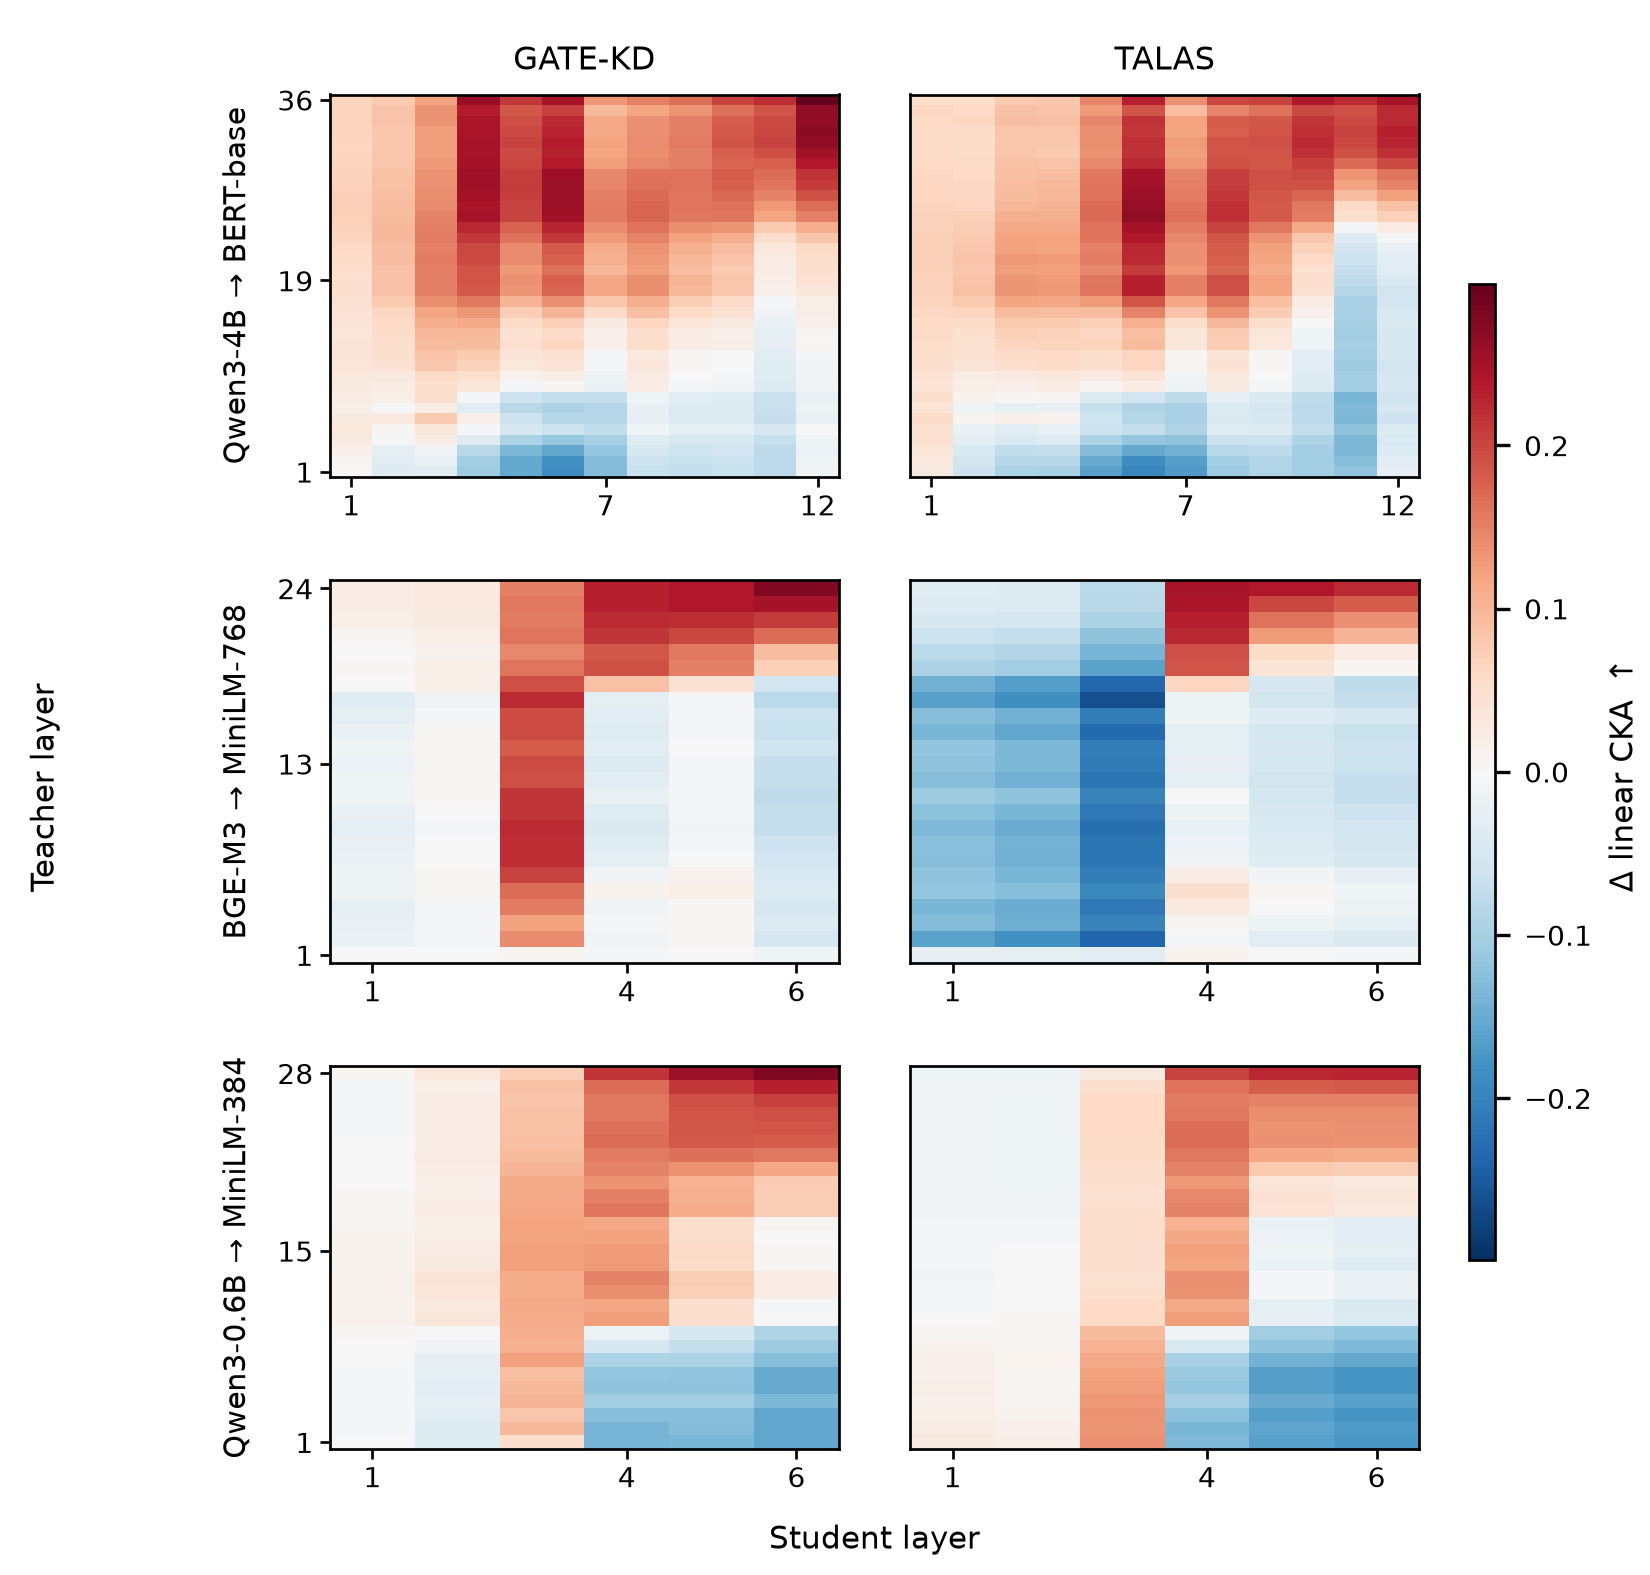
\includegraphics[width=0.82\textwidth]{figures/layerwise_delta_cka_all_pairs}
    \caption{Change in layerwise linear CKA relative to the pretrained
    student. Red and blue denote increased and decreased similarity,
    respectively.}
    \label{fig:layerwise-delta-cka}
\end{figure}

The changes are distributed across multiple later student layers rather than
being confined to a single teacher--student layer pair. This pattern is
consistent with endpoint supervision inducing an internal reorganization of
the student despite the absence of explicit intermediate-layer matching. Some
layer pairs decrease in CKA, so the result does not imply uniformly stronger
alignment at every depth. Moreover, CKA is descriptive and does not establish
that the observed internal changes cause the downstream improvements.

\FloatBarrier
\section{PCA Centering, Whitening, and Random-Subspace Controls}
\label{app:pca-controls}

We isolate preprocessing of the fixed endpoint interface in configuration (c).
Every row uses the endpoint-only objective, the same student, corpus, optimizer,
training schedule, and epoch-wise Procrustes updates. These are endpoint-only
controls, so the reference row is not labeled as GATE-KD or Ours; those names
refer to the full endpoint-plus-$H_0$ method in the main tables. The reference
estimates its principal directions from the centered cache but applies the
resulting linear map without subtracting the cache mean. ``Mean-subtracted
PCA'' applies that
mean subtraction as in the textbook affine PCA transform, while ``PCA
whitening'' additionally rescales each retained coordinate by the inverse square
root of its fitted eigenvalue. The random controls replace the PCA subspace with
three independent Haar-random subspaces of the same rank. Results are averaged
over the same three training seeds within each row; random-map draws remain
separate rather than being treated as additional training seeds.

% Sources: PCA + Procrustes reference from Table 3; remaining rows from
% review_h0_pca_controls_20260906-104859, PCA-family rows only.
\begin{table}[!htbp]
  \centering
  \caption{PCA preprocessing and subspace controls with endpoint-only
  supervision and Procrustes alignment in configuration (c). Scores are mean
  $\pm$ sample standard deviation over three seeds; random-subspace draws are
  shown separately. Best values are bold.}
  \label{tab:pca-preprocessing}
  \small
  \newcommand{\pcell}[2]{#1{\tiny $\pm$ #2}}
  \setlength{\tabcolsep}{4.5pt}
  \begin{tabular}{@{}lcccc@{}}
    \toprule
    Interface & Retained energy $\uparrow$ & Avg. IOD $\uparrow$
    & Avg. OOD $\uparrow$ & Avg. $\uparrow$ \\
    \midrule
    PCA $+$ Procrustes (reference)
      & 0.928 & \pcell{67.76}{0.05} & \pcell{77.54}{0.07}
      & \pcell{\textbf{74.28}}{0.03} \\
    Mean-subtracted PCA
      & 0.928 & \pcell{66.85}{0.15} & \pcell{74.95}{0.02} & \pcell{72.25}{0.06} \\
    PCA whitening
      & 0.928 & \pcell{\textbf{68.14}}{0.33} & \pcell{75.83}{0.08}
      & \pcell{73.26}{0.16} \\
    Random subspace (draw 0)
      & 0.381 & \pcell{67.38}{0.07} & \pcell{77.28}{0.06} & \pcell{73.98}{0.06} \\
    Random subspace (draw 1)
      & 0.376 & \pcell{67.41}{0.17} & \pcell{77.47}{0.05} & \pcell{74.12}{0.04} \\
    Random subspace (draw 2)
      & 0.374 & \pcell{67.48}{0.07} & \pcell{76.95}{0.08} & \pcell{73.79}{0.03} \\
    Uncentered SVD
      & \textbf{0.945} & \pcell{67.59}{0.22}
      & \pcell{\textbf{77.61}}{0.01} & \pcell{74.27}{0.08} \\
    \bottomrule
  \end{tabular}
\end{table}


Mean subtraction causes the largest degradation, particularly on the six OOD
benchmarks. Whitening recovers part of that loss and improves Avg.~IOD over the
reference, but remains lower on Avg.~OOD and overall Avg. The PCA reference
exceeds all three random draws despite retaining the same rank. Uncentered SVD
attains a numerically indistinguishable overall score, differing from the
Table~\ref{tab:interface-families} reference by 0.01 points. We
therefore retain the evaluated interface, while interpreting this control as
evidence for preserving the mean component at application time rather than as
evidence that fit-time centering is uniquely optimal.

\section{Target-Rank Sensitivity at Fixed Student Width}
\label{app:target-rank}

We isolate the subspace selected by the endpoint interface in configuration
(c). The student architecture, 384-dimensional output, distillation corpus,
optimizer, training schedule, and Procrustes updates remain fixed, while the
retained PCA rank varies over $k\in\{64,128,256,384\}$. This experiment uses
the endpoint-only objective. Targets with $k<384$ are embedded in the native
student space by appending zero coordinates before Procrustes alignment. This
padding preserves their Gram matrix and active rank, and does not change the
capacity or width of the student.

Retained energy is measured on the complete teacher cache. On a fixed sample
of 2{,}048 normalized teacher embeddings $T$, we measure the normalized
squared Gram distortion
$\lVert TT^\top-Y_kY_k^\top\rVert_F^2/\lVert TT^\top\rVert_F^2$, where $Y_k$
is the normalized rank-$k$ PCA target. We also report the normalized rank
floor $\sum_{j>k}\sigma_j(T)^4/\sum_j\sigma_j(T)^4$ from
Equation~\ref{eq:gram-lower-bound}. The Gram quantities are independent of
the orthogonal gauge and are therefore computed once, while downstream scores
are averaged over three seeds.

Figure~\ref{fig:target-rank} shows monotonic changes in all three quantities.
Increasing $k$ from 64 to 384 raises retained teacher energy from 59.32\% to
92.84\%, reduces normalized Gram distortion from 6.797\% to 0.086\%, and
improves Avg. from 72.57 to 74.27. The intermediate ranks 128 and 256 attain
73.77 and 74.21 Avg., respectively. Most of the downstream benefit is therefore
recovered by rank 256, with the final increase to rank 384 contributing only
0.06 points in this configuration.

\begin{figure}[H]
    \centering
    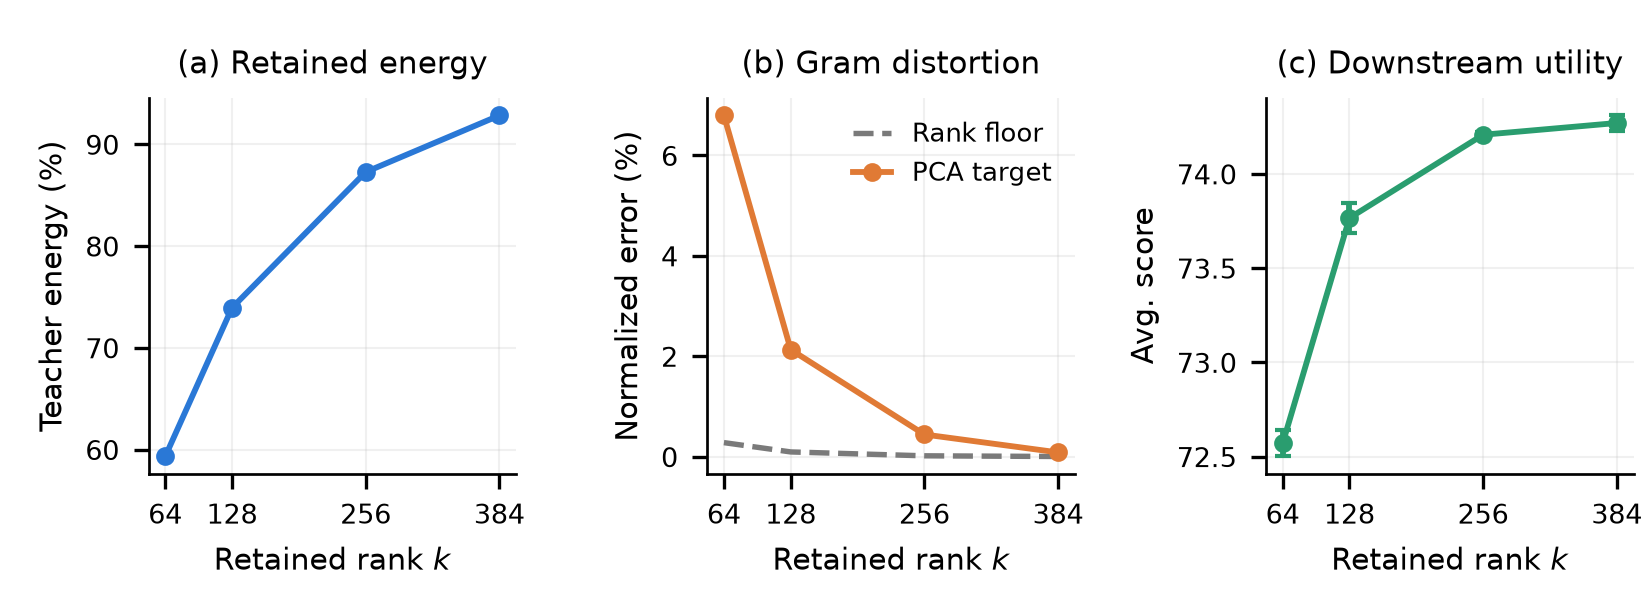
\includegraphics[width=0.85\textwidth]{figures/width_bottleneck}
    \caption{Sensitivity to retained PCA rank at fixed student width in
    configuration (c). Downstream scores show mean $\pm$ sample standard
    deviation over three seeds.}
    \label{fig:target-rank}
\end{figure}

PCA distortion remains roughly 21--25 times above the rank floor because its
objective differs from normalized Gram approximation; the floor bounds
irreducible error rather than predicting this interface's distortion.
Increasing rank improves geometry and utility with diminishing returns. With
the student architecture fixed, this is target-rank sensitivity, not a width
ablation.
